\documentclass[11pt]{article}
\usepackage[english]{babel}
\usepackage[T1]{fontenc}
\usepackage[utf8]{inputenc}
\usepackage{palatino,authblk}
\usepackage[letterpaper,top=2cm,bottom=2cm,left=2.6cm,right=2.6cm]{geometry}
\usepackage{amsmath,amssymb,booktabs,array,microtype,graphicx}
\usepackage[colorlinks=true,allcolors=blue]{hyperref}
\setlength{\parskip}{3pt}
\title{\vspace{-1.3cm}Selecting Reliable LLM Reasoning\\[3pt]\large Candidate-Set Attention with a Linear Ranking Ensemble\\[3pt]\normalsize DASE7506 Advanced Machine Learning Methods --- MP2}
\author[*]{\small Zheng Qiaoyi 3036801242}
\affil[*]{\small  Robotics and Intelligent Systems, DASE}
\date{}
\begin{document}
\maketitle
\vspace{-0.8cm}

\begin{abstract}
This project selects one of four supplied mathematical solutions using fixed embeddings, numerical and textual features, and comparison across candidates. The frozen method combines three candidate-set attention networks with a pairwise linear ranker and pools scores for equivalent final answers. The supplied official-score JSON records 389 correct selections out of 467 test questions (83.2976\%). A saved local measurement records 1.6455 seconds for prediction and scoring; the inference assets occupy 4.7409 MiB. These are existing project records, not newly reproduced measurements. Historical comparisons suggest improvement over the initial model, but missing ablations prevent attribution to individual components.
\end{abstract}

\section{Task and research question}
The course benchmark contains 4,755 training, 798 validation, and 467 test questions, each with four candidate solutions and a $4\times1024$ array of fixed representations. At least one candidate has the correct final answer. Test groups contain at least two distinct valid parsed answers, whereas training and validation include easier groups. The output is a candidate index, and the fixed evaluator compares its parsed final numeric answer with the reference. It does not certify every reasoning step.

The motivating hypothesis is that comparing solutions within a question can improve selection over judging each candidate independently. Agreement, relative features, and attention can provide complementary evidence, but agreement can also reinforce shared errors. A compact linear ranker provides a second scoring mechanism. The available records support comparison of complete versions; they do not isolate the causal benefit of attention, arithmetic checks, or fusion.

\section{Implemented method}
\subsection{Representations and numerical checks}
The feature extractor constructs 35 scalar features per candidate: parsing validity, answer agreement and diversity, answer magnitude/sign/integrality, text length and relative length, token and formatting counts, question length, and 21 lexical counts. It concatenates these with the 1024-dimensional supplied embedding and its deviation from the four-candidate mean, giving 2083 features for the linear ranker.

The attention input selects the 35 scalar features and the original 1024 embedding dimensions, then adds eight arithmetic-check features, giving 1067 dimensions. Thus, the attention and ranking branches do not use identical inputs. Arithmetic checks normalize selected multiplication, division, and fraction notation and inspect a restricted class of explicit numerical equalities. Features include checked-equation counts, disagreement counts, relative-error summaries, and coverage. They cannot verify symbolic algebra or whether an equation correctly models the question. A correct multiplication can still implement an incorrect interpretation.

For the attention branch, training-fitted means and scales standardize each feature; values are clipped to $[-8,8]$. The ranker uses its own training-fitted standardization without this clipping. Both transformations are stored with the frozen assets.

\subsection{Candidate-set attention}
Each model projects a four-candidate feature matrix to width 128, applies two transformer encoder layers with four heads, and produces a scalar logit per candidate. Each layer uses a feed-forward width of 256, GELU, pre-normalization, and dropout 0.3. A direct linear skip branch adds an input-based score. There is no positional encoding, so the network can compare the candidate set without explicitly encoding candidate order. Equal-score selection can still depend on the final argmax tie-breaking rule.

Let $s_i$ be the logit of candidate $i$, $V$ the valid parsed candidates, and $C\subseteq V$ the correct candidates. Training combines
\begin{align}
L_{\rm pair}&=\frac{1}{|P|}\sum_{(i,j)\in P}\log(1+\exp(-(s_i-s_j))),\\
L_{\rm mass}&=\log\sum_{i\in V}\exp s_i-\log\sum_{i\in C}\exp s_i,\\
L&=0.5L_{\rm pair}+0.5L_{\rm mass}+0.15L_{\rm BCE},
\end{align}
where $P$ contains correct--incorrect valid pairs. For groups without such pairs, the implemented pair term is zero. Binary cross-entropy is averaged over candidate logits. The mass term accommodates multiple correct choices rather than arbitrarily treating one correct candidate as the sole target.

Three networks use seeds 42, 123, and 2026. Each is trained for five epochs with AdamW, learning rate $10^{-4}$, weight decay 0.08, batches of approximately 64 questions, and gradient norm clipping at 3. These are three initializations of the same architecture, not three distinct architectures. The fixed training script reports validation results without changing its recipe.

\subsection{Linear ranking, fusion, and answer pooling}
The linear model learns from standardized differences between correct and incorrect candidate features. Both each difference and its negation are included with opposite binary labels. It uses logistic regression with $C=0.001$, no fitted intercept, and a maximum of 2000 iterations. Candidate logits are converted to probabilities by a masked softmax.

At inference, the attention probabilities are averaged across seeds and combined with ranking probabilities:
\begin{equation}
p_i=0.75\left(\frac{1}{3}\sum_{k=1}^{3}p_i^{(k)}\right)+0.25p_i^{\rm rank}.
\end{equation}
For each group $G(a)$ of candidates with the same parsed answer $a$, the configuration sets every member's score to
\begin{equation}
\widetilde p_i=\frac{1}{|G(a)|}\sum_{j\in G(a)}p_j,\qquad i\in G(a).
\end{equation}
This is mean pooling, not summation of the group's probability mass. Invalid candidates are excluded before selecting the largest pooled score. The returned object remains one candidate index; the method generates no new answer.

\section{Results and strength of evidence}
\begin{table}[ht]
\centering\small
\begin{tabular}{lrrl}
\toprule
Method & Correct / 467 & Accuracy & Evidence\\
\midrule
Initial CatBoost & 365 & 78.1585\% & README only\\
Linear + small MLP fusion & 379 & 81.1563\% & README only\\
Looped attention + Brier & 385 & 82.4411\% & README only\\
Final attention + ranker & 389 & 83.2976\% & Score JSON + assets\\
\bottomrule
\end{tabular}
\caption{Recorded complete-test-bank results. Historical methods were not rerun for this report; their detailed logs and checkpoints are absent from this folder.}
\end{table}
\begin{figure}[ht]
\centering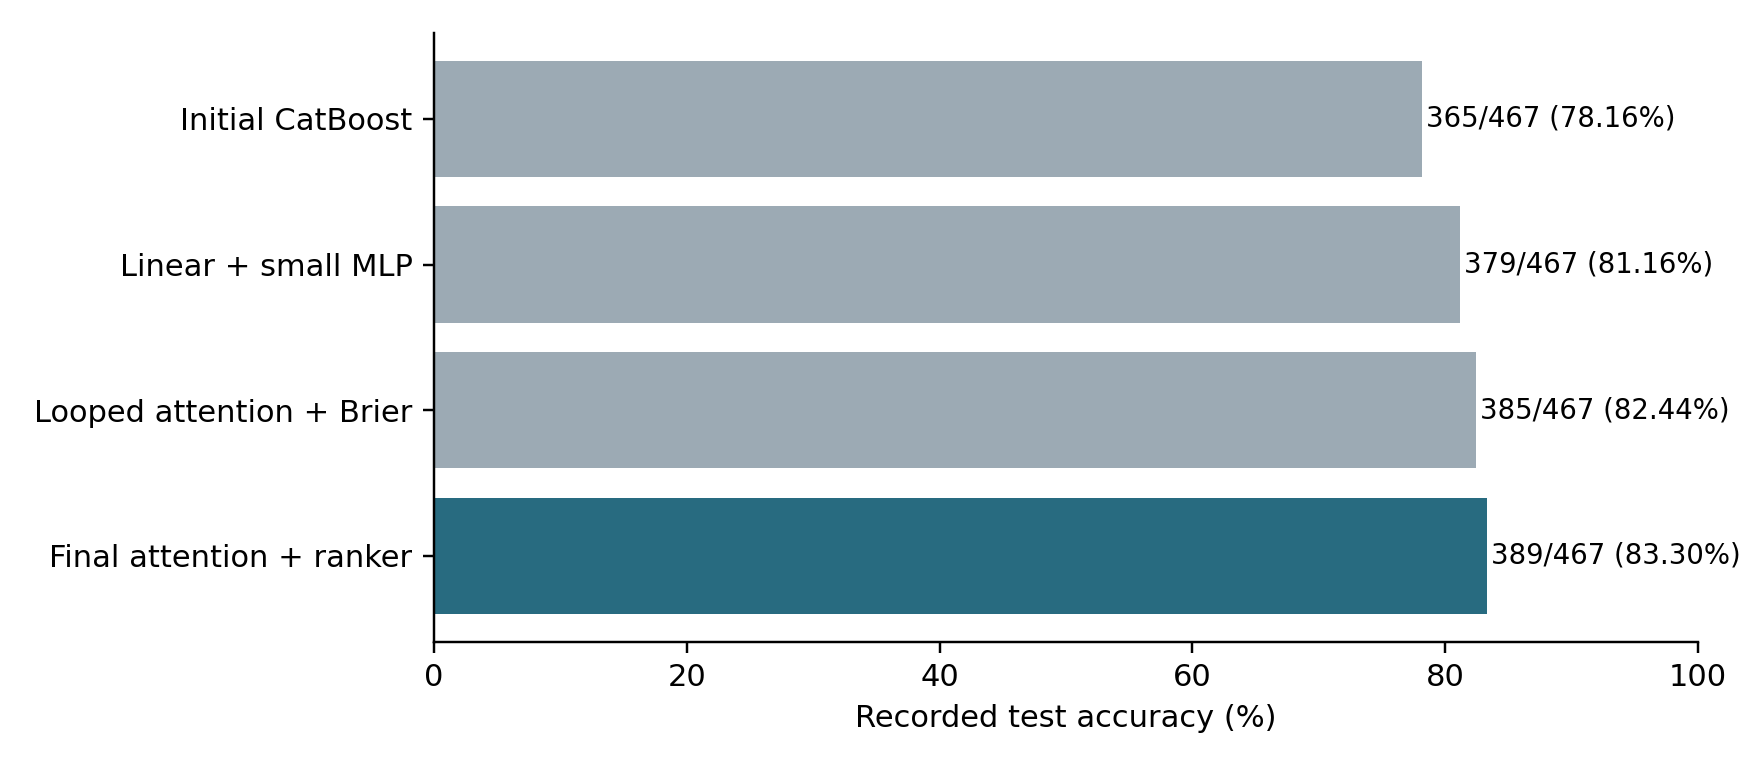
\includegraphics[width=0.94\textwidth]{figures/results.png}
\caption{Visualization of the recorded counts. This is a comparison of versions, not a controlled component ablation.}
\end{figure}

The final version selects 24 more correct answers than the initial CatBoost version, an increase of 5.1392 percentage points. It improves on the linear/MLP version by 10 answers (2.1413 points). Relative to the looped-attention experiment, the difference is only four answers (0.8565 points). Without paired predictions for the other methods, statistical significance and overlap in errors cannot be established.

The configuration records validation accuracy 0.9385964912 and hard-validation accuracy 0.8619718310. These are saved metadata, not freshly reproduced scores; the exact hard-subset construction is not documented in the provided final training script. The easier groups in validation also mean that full-validation accuracy should not be compared directly with test accuracy as if both distributions were identical.

The README reports that answer grouping, arithmetic verification, hard-negative approaches, and out-of-fold fusion did not yield stable validation improvements in earlier experiments. It supplies no quantitative ablation table. Consequently, this report does not invent an attention-only score, an arithmetic-free score, or a fusion gain. A proper follow-up would freeze the protocol, compare these variants on validation, and reserve a separate audit bank for final generalization assessment.

\subsection{Test exposure and limitations}
The project README explicitly states that aggregate scores on the same test bank were inspected and used to compare evaluated versions. It also states that test labels, per-question test errors, and answer lookup tables were not used for training. Inspection of the provided fixed training path is consistent with training on training references and reporting validation performance, but it cannot reconstruct the entire historical development process.

Aggregate test-based model selection can still bias the final estimate and conflicts with a strict separation of test scoring from method selection. The result should therefore be described as the recorded best evaluated score on this public course bank, with that exposure disclosed. An unseen audit bank would provide stronger evidence of generalization.

There are 78 incorrect final selections, but the folder does not include the original questions and references needed for a grounded per-example error analysis. Plausible failure mechanisms include confidently worded incorrect solutions, shared wrong answers, missed semantic conditions, and arithmetic expressions outside the restricted checker. These are hypotheses, not observed counts of error categories. Softmax outputs and ensemble agreement have not been shown to be calibrated confidence estimates.

\section{Resources and reproducibility}
The five checkpoint files total 4,970,167 bytes, or approximately 4.7409 MiB, below the 16 MiB asset limit. The saved external timing is 1.6454782 seconds for the fresh prediction and independent scoring subprocesses. The scorer-only time is 0.0162541 seconds and must not be confused with end-to-end evaluation time. The README identifies the local hardware as an Intel Core i7-13700KF and Python 3.12.10. Reference-machine eligibility still requires measurement on the specified Xeon Platinum 8457C.

The launcher sets thread-related environment variables to four, and prediction sets PyTorch threads to four. Its timer begins after launcher-side manifest verification and includes the two child processes. The supplied record does not independently audit actual thread usage. Training uses 15 network epochs in total across three seeds, plus a linear fit; complete historical search time and training hardware records are not available here.

\begin{table}[ht]
\centering\small
\begin{tabular}{lr}
\toprule
Inference asset & Bytes\\
\midrule
\texttt{attention\_42.pt} & 1,639,602\\
\texttt{attention\_123.pt} & 1,639,638\\
\texttt{attention\_2026.pt} & 1,639,674\\
\texttt{rank.npz} & 50,994\\
\texttt{config.json} & 259\\
\midrule
Total & 4,970,167\\
\bottomrule
\end{tabular}
\caption{All five files in \texttt{code/checkpoint} are required to reproduce the submitted method without retraining.}
\end{table}

From the supplied project root, evaluation is intended to use the following commands, with an external copy of the unmodified official data:
\begin{verbatim}
python -m pip install -r code/requirements.txt
python code/run.py --data-dir "PATH/TO/OFFICIAL/data"
\end{verbatim}
The inference requirements pin NumPy 2.2.6 and CPU PyTorch 2.5.1. Training dependencies are separately recorded in \texttt{requirements-training-lock.txt}; the CPU wheel index is required as specified there. For fixed-recipe retraining in PowerShell:
\begin{verbatim}
$env:MP2_DATA_DIR="PATH/TO/OFFICIAL/data"
python code/train_fixed.py
\end{verbatim}
The output is \texttt{code/retrained\_checkpoint}, preserving the frozen assets. The saved retraining-check file contains true flags for the three seeds and ranker, but does not specify the comparison procedure or tolerance; it is not sufficient by itself to claim cross-platform bitwise reproducibility.

The scanned folder lacks official data and the historical reports referenced in its README. Some README commands also refer to an earlier \texttt{FINAL\_SUBMISSION} layout. The commands above match the current \texttt{code} layout. No evaluation or training was rerun while preparing this report. \texttt{MANIFEST.json} provides SHA256 entries for the frozen implementation and assets; any edited code version should be accompanied by updated version identification and a matching manifest.

\section{AI assistance, reuse, and conclusion}

\textbf{This report, its result figure, and its explanatory analysis were generated by Codex AI.} The underlying project likewise records substantive AI assistance with implementation and experiments. AI-generated prose does not supply missing experimental evidence, and no unsupported ablation results or new measurements have been added.

The frozen system demonstrates a compact implementation of candidate comparison and ensemble ranking, with a recorded accuracy of 83.2976\% and modest local inference cost. The evidence supports the reported frozen result more strongly than it supports claims about which component caused the improvement. Missing controlled ablations and prior test-score exposure remain material limitations. The main next step is a validation-only component comparison followed by independent audit-bank evaluation.
\end{document}
